\documentclass[a3paper]{article}
\usepackage[left=0cm,top=1in,right=0mm,bottom=0mm]{geometry}
\usepackage{tikz}
\begin{document}
\centering
\Huge\textbf{How to Play the Game?}
\vspace{2in}
\begin{center}
\LARGE
    \begin{enumerate}
    \item[Step 1.]{Roll a pair of dice.}
    \item[Step 2.]{Add the numbers shown on the dice.}
    \item[Step 3.]{Record the total by placing a mark on the chart.}
\end{enumerate}
\end{center}
\newpage
\centering
\begin{tikzpicture}[scale=1]
    \draw (\textwidth/6,-1) grid[step=\textwidth/12] ({13\textwidth/12},\textwidth);
    % \clip (-10.5,3) rectangle (10.5,{-21*sqrt(2)-3});
    \foreach \n in {2,...,12}{
    %   \foreach \x in {0,...,\y}{
    \node[xshift=\textwidth/24] at ({(\n)*\textwidth/12},-1) {\n};
    %     \draw ({\y/2-\x},{-\y*sqrt(3)/2}) circle (0.5);
    %   }
    }    
    \draw[ultra thick] (\textwidth/6,0) -- ({13\textwidth/12},0) node[midway,yshift=-1.5cm] {Sum};
    \draw[ultra thick,->] (\textwidth/6,0) -- ({\textwidth/6},0.8\textheight) node[sloped,midway,above] {Frequency (Number of times the sum appears)};
\end{tikzpicture}
\end{document}